\documentclass{report}

% Matemática
\usepackage{amsmath}    % símbolos matemáticos
\usepackage{amsthm}     % teoremas
\usepackage{amsfonts}   % \mathbb
\usepackage{bm}         % bold math (https://ctan.org/pkg/bm)


% Figuras
\usepackage{tikz}                   % gráficos
\usepackage{float}                  % [H]
\usepackage{xcolor}                 % colores https://es.overleaf.com/learn/latex/Using_colours_in_LaTeX

% Texto
\usepackage[shortlabels]{enumitem}  % enumerate con letras


\usetikzlibrary{arrows,positioning,automata,shadows,fit,shapes}

% Teoremas, corolarios, etc.
% https://www.overleaf.com/learn/latex/theorems_and_proofs
\theoremstyle{definition} % Para que no salga en italicas

\newtheorem{theorem}{Teorema}
\newtheorem*{theorem*}{Teorema}

\newtheorem{lemma}{Lema}
\newtheorem*{lemma*}{Lema}

\newtheorem{proposition}{Prop.}
\newtheorem*{proposition*}{Prop}

\newtheorem{definition}{Def.}
\newtheorem*{definition*}{Def}

\author{Manuel Panichelli}
\title{Notas de \\\textit{Algoritmos, Azar y Autómatas}}

\begin{document}
\maketitle

\chapter{Introducción}

\section{Azar}

Azar es \textbf{imposibilidad de predecir}, \textbf{falta de patrones},
imposibilidad de abreviar, comprimir.

Vamos a categorizar el azar según diferentes modelos de cómputo

\begin{itemize}
    \item Autómatas finitos
    \item Autómatas de pila
    \item Máquinas de turing
\end{itemize}

\begin{definition}
    Una secuencia es \textbf{azarosa} (para los autómatas de la clase $C$)
    cuando, esencialmente, la única forma de describirla (mediante un autómata
    de la clase $C$) es nombrando explícitamente cada uno de sus símbolos.
\end{definition}

Esto quiere decir que no tiene patrones (porque sino podríamos nombrar menos) y
que no se puede comprimir. \textit{Esencialmente} porque se pueden hacer
pequeñas conversiones. Por ejemplo, las cadenas de $\{a^n b^n \mid n \in
\mathbb{N}\}$ son azarosas para AF pero no para AP (porque es un lenguaje libre
de contexto pero no regular).

Hay distintos \textit{grados de azar}:

\begin{enumerate}
    \item \textbf{Azar puro}: Impredecibilidad / incompresibilidad para
    máquinas de turing
    \item \textbf{Azar básico}: Impredicibilidad / incompresibilidad para
    autómatas finitos.
\end{enumerate}

\begin{enumerate}
    \item Una secuencia es \textbf{random} si, esencialmente, sus
    \textit{segmentos iniciales} solo se pueden describir explícitamente por una
    Turing Machine (no pueden ser comprimidos por una TM)
    \item Una secuencia es \textbf{normal} si, esencialmente, sus segmentos
    iniciales solo se pueden describir explicitamente por un autómata finito.
\end{enumerate}

Cosas que no copié

\begin{enumerate}
    \item Kolmogorov / program size complexity
    \item Definicion de azar de Chaitin basado en kolmogorov
    \item Martin Löf random
\end{enumerate}

\section{Numeros normales}

\begin{definition*}
    Una \textbf{base} es un entero $\geq 2$. Para un $x \in \mathbb{R}$ en el
    intervalo unitario\footnote{El intervalo unitario es el intervalo cerrado
    $[0, 1]$}, su \textbf{expansión} en base $b$ es una \textbf{secuencia} $a_1
    a_2 a_3 \dots$ de enteros de ${0, 1, \dots, b-1}$ tales que

    $$x = 0.a_1 a_2 a_3 \dots,$$

    donde $x = \sum_{k \geq 1} \frac{a_k}{b_k}$ y $x$ no termina con una cola de
    $b - 1$ (esto lo hacemos para tener una representación única de todos los
    numeros racionales)

    Cuando se de por sentada la base $b$ denotamos los primeros $n$ digitos de
    la expansión de $x$ con $x[1\dots n]$
\end{definition*}


\begin{definition}[Números normales, Borel 1909]
    Un número real $x$ es,
    \begin{itemize}
        \item \textbf{Simplemente normal a base $b$} si en la expansión de $x$
        en base $b$, cada digito ocurre con una frecuencia de $1/b$ en el
        límite.

        \textit{(En el límite todos los símbolos tienen la misma frecuencia)}
        \item \textbf{Normal a base $b$} si para cada entero positivo $k$, cada
        bloque de $k$ digitos (arrancando de cualquier posición) ocurre en la
        expansión de $x$ en base $b$ con una frecuencia en el límite de $1/b^k$
        \item \textbf{Absolutamente normal} si es normal para todas las bases.
    \end{itemize}
\end{definition}

Ejemplos:

\begin{itemize}
    \item $0.01 \ 002 \ 0003 \ 00004 \ 000005 \ 0000006 \ 00000007 \ 000000008 \dots$
    no es simplemente normal a base $10$ (el 0 tiene más frecuencia que el
    resto)
    \item $0.0123456789 \ 0.0123456789 \ 0.0123456789 \ 0.0123456789 \dots$ es
    simpelemente normal a base $10$, pero no es simplemente normal a base 100.

    \textit{Pasar de base 10 a base 100 es tomar combinaciones de dos dígitos en base 10 de forma contigua}

    \item El ternario de cantor no es simplemente normal a base 3 (las
    expansiones no tienen el dígito 1)

    \item Los numeros racionales no son normales a ninguna base
    
    Si agarro un número racional, por ej 3.14

    $$3.14 \rightsquigarrow 3.140000000\dots$$
    
    en base 10 tiene un período que se repite

    \item La constante de Liouville $\sum_{n \geq 1} 10^{-n!}$ no es normal a
    base 10
\end{itemize}

\begin{theorem}[Borel 1909]
    Casi todos los números reales son absolutamente normales.
\end{theorem}

Son las constantes matemáticas usuales como $\pi$, $e$ o $\sqrt{2}$
absolutamente normales? O al menos simplemente normales a alguna base? Es una
pregunta abierta.

\begin{theorem}[Champernowne, 1933]

    Todos los numeros naturales en base 10 concatenados es normal a base 10.

    $$0.123456789101112131415161718192021\dots$$

    \textit{No se sabe si es normal a bases que no son potencias de 10}
    
\end{theorem}

\begin{theorem}[Cassels 1959; Schmidth 1961]
    Casi todos los números del ternario de Cantor son normales a base 2.
\end{theorem}

\begin{theorem}[Bailey y Borwein 2012]
    El número de Stoneham $\alpha_{2, 3} = \sum_{k \geq 1} \frac{1}{3^k
    2^{3^k}}$ es normal a base 2 pero no simplemente normal a base 6.
\end{theorem}

\subsection{Normalidad y autómatas finitos}

\begin{definition}
    Una secuencia $x = a_1 a_2 a_3 \dots$ es \textbf{compresible} por un
    trasductor finito $T$ si y solo si en la corrida en $T$ $q_0
    \xrightarrow{a_1\mid v_1} q_1 \xrightarrow{a_2\mid v_2} q_2
    \xrightarrow{a_3\mid v_3} q_3 \dots$ satisface que

    $$\underset{n \to \infty}{\text{lim inf}}\ \frac{|v_1 v_2 \dots v_n|}{n} <
    1.$$
    
    \textit{Recordar que los $a$ son símbolols y los $v$ cadenas, posiblemente vacías.}
\end{definition}

\begin{theorem}
    Una secuencia es \textbf{normal} si y solo si es \textbf{incompresible por
    todo one-to-one transducer}.
\end{theorem}

\begin{theorem*}[Becher, Casrton, Heiber 2013]
    Los transductores finitos uno a uno no deterministicos con contadores no
    pueden comprimir secuencias normales.
\end{theorem*}

\begin{theorem*}
    
\end{theorem*}
    Los trasductores de pila no determinísticos pueden comprimir secuencias
    normales.
    
    $$
        0123456789\ \textcolor{blue}{9876543210}\
        00\ 01\ 02\ 03 \dots 98\ 99\ \textcolor{blue}{99\ 98\ 97 \dots 03\ 02\ 01\ 00\ }
        000\ 001\ 002 \dots
    $$

    \textit{Va pusheando y cuando detecta el cambio empieza a desapilar.
    Parecido al APD que reconoce $w\#w^r$}

\chapter{3 secuencias normales}

\section{Notación}

\begin{itemize}
    \item Un \textit{alfabeto} es un conjunto finito de símbolos. Por ej $A$
    \item $A^\omega$ es el conjunto de todas las palabras infinitas
    \item $A^*$ (la clausura de Kleene) es el conjunto de todas las palabras finitas
    \item $A^{\leq k}$ es el conjunto de todas las palabras de longitud hasta $k$
    \item $A^{k}$ es el conjunto de palabras de longitud exactamente $k$.
    \item Si $w$ es una cadena $|w|$ es su longitud.
    \item Las posiciones de las cadenas se numeran desde 1
    \item $w[i]$ es el simbolo iésimo de $w$ y $w[i\dots j]$ es el substring de
    $i$ a $j$.
    \item La cadena vacía es $\lambda$
\end{itemize}

\begin{definition}
    El número de ocurrencias alineadas y no alineadas de una cadena es

    \begin{align*}
        |w|_u &= |\{ i : w[i\dots i+|u| - 1] = u\}|,\\
        ||w||_u &= |\{ i : w[i\dots i+|u| - 1] = u \text{ y } i \equiv 1 \text{ mod } |u|\}|
    \end{align*}

    Por ejemplo, $|aaaaa|_{aa} = 4$ y $||aaaaa||_{aa} = 2$.

    Cuando $u$ es un símbolo las definiciones coinciden. Y la de alineadas son
    posiciones que son múltiplos de $|u|$

    \textit{(La de alineadas tiene $\equiv 1$ en vez de $\equiv 0$ ya que las posiciones se numeran de 1)}
\end{definition}

\begin{proposition*}
    Las ocurrencias alineadas de una palabra de longitud $r$ sobre un alfabeto
    $A$ coinciden con las ocurrencias del símbolo correspondiente sobre el
    alfabeto $A^r$.
\end{proposition*}
\begin{proof}
    Sean un alfabeto $A$, una longitud $r$ y un alfabeto $B$ con $|A|^r$
    símbolos (la cantidad de símbolos que tiene el alfabeto $A^r$). $A^r$ (el
    conjunto de palabras de longitud $r$ sobre el alfabeto $A$) y $B$ son
    isomorfos, existe

    $$\pi: A^r \to B$$

    que se induce del orden lexicográfico en cada conjunto (se puede hacer un
    matching 1 a 1). Por lo tanto, para cada $w \in A^*$ tal que $|w|$ es
    múltiplo de $r$,

    $$|\pi(w)| = |w| / r.$$

    (Una palabra de longitud múltiplo de $r$ es una cadena de $r$ símbolos de
    $A^r$, luego la longitud de la palabra en $B$ que tiene símbolos unitarios
    digamos es esa).

    Luego,

    $$\forall u \in A^r \ (||w||_u = |\pi(w)|_{\pi(u)}).$$
\end{proof}

Por ejemplo, sean $A = \{0, 1\}$, $r = 3$, y $B$ tal que $|A^r| = |B|$,

$$B = \{
    \underset{000}{0},
    \underset{001}{1},
    \underset{010}{2},
    \underset{011}{3},
    \underset{100}{4},
    \underset{101}{5},
    \underset{110}{6},
    \underset{111}{7}
\}$$

Luego la cadena,

$$100\ 100\ 111\ 000$$
$$4470$$

La cantidad de ocurrencias de $100$ coinciden con las de $4$.

\begin{definition}[Normalidad no alineada, Borel]
    Un número real $x$ es \textbf{normal a base $\bm{b}$} si para cada bloque
    $u$,

    $$
    \underset{n \to \infty}{lim}
        \frac{|x[1\dots n]|_u}{n} =
        \frac{1}{b^{|u|}}.
    $$

    \textit{En el límite,como $b^{|u|}$ son todos los bloques posibles de
    longitud $|u|$, $1/b^{|u|}$ seria que cada uno tiene la misma frecuencia.}
\end{definition}

\begin{theorem}[Piatetski-Shapiro 1957]
    Sea $x$ un número real, $b \geq 2$ un entero y $A = \{0, \dots, b - 1\}$.
    Las siguientes son equivalentes
    \begin{enumerate}
        \item $x$ es normal a base $b$
        \item Existe una constante $C$ tal que para infinitas longitudes $\ell$ y
        para todo $w \in A^\ell$

        $$
            \underset{n \to \infty}{\text{lim sum}}
            \frac{|x[1\dots n]|_w}{n} < C \cdot b^{-\ell}.
        $$
        \item Existe una constante $C$ tal que para infinitas longitudes $\ell$ y
        para todo $w \in A^\ell$

        $$
            \underset{n \to \infty}{\text{lim sum}}
            \frac{||x[1\dots n\ell]||_w}{n} < C \cdot b^{-\ell}.
        $$ 
    \end{enumerate}
\end{theorem}

Para el ejercicio hay que hacer la 3ra.

\section{Tres secuencias normales}

\begin{itemize}
    \item Secuencias de Brujin infinitas
    \item A la Champernowne (binario)
    
    $$01\ \ 00\ 01\ 10\ 11\ \ 000\ 001\ 010\ 011\ 100\ 101\ 110\ 111\ \ 0000 \dots$$

    \item Una secuencia normal tal que la subsecuencia en las posiciones pares
    es idéntica a toda la secuencia.
\end{itemize}

\section{De Brujin}

\begin{definition}[De Brujin 1946]
    Definiciones de De Brujin,
    \begin{itemize}
        \item Un \textbf{collar de De Brujin} de orden $n$ sobre un alfabeto $A$
        es una secuencia cíclica de longitud $|A|^n$ tal que cada palabra de
        longitud $n$ ocurre en ella exactamente una vez.

        Ejemplos: 01; 0011; 00011101 (el 100 está en la pos 8 por ej.).

        \item Una \textbf{palabra de De Brujin} (no cíclica) de orden $n$ sobre
        el alfabeto $A$ es una palabra de longitud $|A|^n + n - 1$ (se le agrega
        todo lo que uno podría hacer con un ciclo) tal que cada palabra de
        longitud $n$ ocurre en ella exactamente una vez.

        Ejemplos: 01; 00110; 0001110100.

        \item Una \textbf{palabra infinita de De Brujin} $w = a_1 a_2 \dots$ en
        un alfabeto de al menos tres símbolos es una palabra infinita tal que,

        $$\forall{n}.\ a_1\dots a_{|A|^n + n - 1}$$

        es una palabra de De Brujin de orden $n$.

        Ejemplo: 012, una palabra de De Brujin de orden 1, se puede extender a
        la siguiente de orden 2: 0122002110.

        Si el alfabeto tiene dos símbolos, una palabra infinita de De Brujin $w
        = a_1 a_2 \dots$ es aquella que para cada $n$ impar, $a_1\dots a_{|A|^n
        + n - 1}$ es una palabra de De Brujin de orden $n$.
    \end{itemize}
\end{definition}

\begin{definition}
    Un \textbf{grafo de De Brujin} $G_A(n)$ es un digrafo cuyos vértices son
    palabras de longitud $n$ sobre el alfabeto $A$ y sus ejes los pares $(au,
    ub)$ para alguna palabra $u$ de longitud $n - 1$ y posiblemente dos símbolos
    diferentes $a, b$.

    \begin{figure}[H]
        \centering
        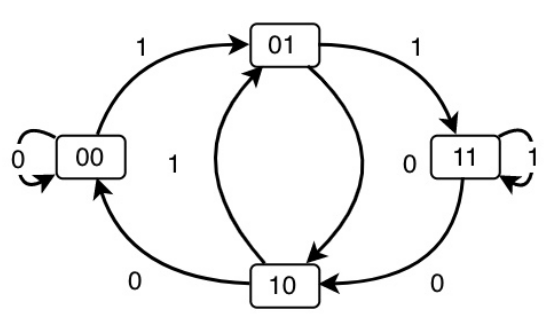
\includegraphics[scale=0.3]{img/2_de_brujin_01.png}
        \caption{Ejemplo de grafo de De Brujin de orden 2 para $A = \{0, 1\}$}
    \end{figure}
    
    \begin{itemize}
        \item Tiene $|A|^n$ vertices y $|A|^{n+1}$ arcos
        \item Es \textit{fuertemente conexo} (existe un camino dirigido entre
        todo par de vértices)\footnote{Conexo a secas en digrafos es que el grafo
        subyacente (sacándole direcicones) sea conexo}
        \item Es \textit{regular}, $\forall v. d_{in}(v) = d_{out}(v)$ (los
        loops suman uno a la entrada y salida)
        \item Es Euleriano (por teorema de Euler, solo hace falta que sea
        regular y fuertemente conexo).
    \end{itemize}
\end{definition}

\begin{figure}[H]
    \centering
    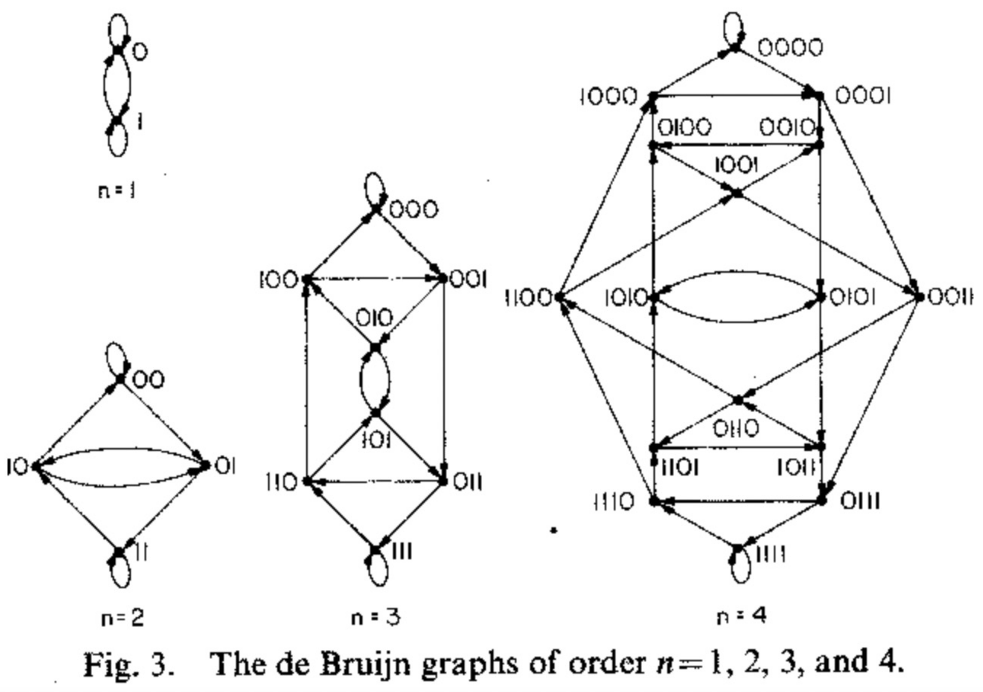
\includegraphics[scale=0.3]{img/2_de_brujin_ord_1234.png}
    \caption{Grafos de De Brujin de ordenes 1, 2, 3 y 4 sobre $A = \{0, 1\}$}
\end{figure}

\begin{definition*}
    El \textbf{grafo de línea} de un grafo $G$, es otro grafo que tiene como
    vértilos ejes de $G$ y como ejes los caminos de longitud 2.
\end{definition*}


\begin{proposition}
    Toda secuencia de De Brujin de orden $n+1$ sobre un alfabeto de $|A|$
    simbolos se puede construir como un ciclo Euleriano en $G_A(n)$.
\end{proposition}

\begin{proposition}[Becher, Heiber 2011]\label{prop:de-brujin-extend}
    Dado un alfabeto $A$ con al menos tres símbolos, toda secuencia de De
    Brujin de orden $n$ se puede extender a una de orden $n + 1$
\end{proposition}
\begin{proof}
    Dado un alfabeto $A$, suponiendo que $E$ es un ciclo Euleriano de $G_A(n)$.
    Como $G_A(n + 1)$ es el grafo de línea de $G_A(n)$, $E$ es un ciclo
    Hamiltoniano en $G_A(n+1)$.

    \textit{Está la demo en las clases, no la terminé de ver.}

    \textit{Todo ciclo euleriano va a ser hamiltoniano en el grafo de línea, porque los vertices son los ejes}
\end{proof}

Para computar una palabra infinita de De Brujin puedo para cada $n \geq 1$
extender un ciclo Hamiltoniano en un grafo de De Brujin de orden $n$ a uno
Euleriano en el mismo grafo. Esto se hace en tiempo exponencial de $n$, y no se
conoce ningun algoritmo eficiente.

\begin{theorem}[Ugalde 2000]
    Las palabras infinitas de De Brujin son normales.

    Si el alfabeto $A$ tiene dos símbolos, se puede considerar el alfabeto $A'$
    de 4 símbolos que se obtiene con el morfismo que mapea bloques de dos
    simbolos en $A$ a un simbolo en $A'$ y probar normalidad ahí.
\end{theorem}

\end{document}
